\documentclass[a4paper]{article}
 
\usepackage{amsmath}
\usepackage{graphicx}
\usepackage{caption}
\usepackage{subfigure}
\usepackage{epstopdf}
\usepackage[ansinew]{inputenc}
\usepackage{listings}
\usepackage{xcolor}
%\setlength{\oddsidemargin}{0cm}
%\setlength{\evensidemargin}{0cm}
%\setlength{\topmargin}{0cm}

\usepackage[]{algorithm2e}

\usepackage{a4wide}

\title{Process connection information for neurons on the fly using MPI}
\author{BBP}
%\date{}

\begin{document}
   \maketitle


\section{Algorithms}
The given data file format (Figure \ref{Mikesformatcon}) stores the connections by source neurons.
NEST stores the connection information on the post-synaptic side of the nodes (by target neuron).
Also the \emph{Connect} functions have to be called from the post-synaptic nodes.
To reduce the amount of IO, reading of the data files should be done in parallel.
Each node should read a defined amount of HDF5 files, process it and send it to the corresponding node,
to deliver the connection information to the nodes (where the target neuron is) MPI is used.
Depending on the distribution of the data, different algorithms and data structures can be used.
Two possible algorithms are listed below. The main difference is the data structure which is sent via MPI.
The choice for the optimal algorithm depends on the ratio of source and target neurons in the chunks.
Both algorithm uses the \emph{MPI\_Alltoall} function. The function distribute data from each node to all other nodes.
Therefore each node has to be able to create the mapping of target neurons to nodes.
For \emph{NEST} this is possible, because the mapping is based on an explicit function.
If this is not the case \emph{MPI\_Allgather} can be used.
So all connection data is distributed to all nodes and each node can extract its data.


\section{Group data before send}
The group data before send algorithm reads the the HDF5 file chunk wise.
Additionally the source neurons for each datasets (first row) are stored in a list.
So for all iterations the source neuron list is available in memory.
This source neuron list and the target neurons from each chunk are used to create a connection table.
It contains per connection one row with the source neuron in the first column and the target neuron in the second column.
The table will be sorted by the target nodes.
Using the \emph{MPI\_Alltoall} function this table can be distributed directly to the corresponding nodes.
Afterwards each node contains its connection table and calls the \emph{NEST} connection function.
\begin{algorithm}
	\KwData{List of HDF5 files for each node, chunk size}
	\KwResult{Connected NEST network}
	\While{Chunk to read in HDF5 files}{
		Read chunk and store in memory \hspace{45px}(1)\; 
		Create connection table [[$S_1$, $T_1$],[$S_2$, $T_2$],..] (1,2) \hspace{36px}$\mathcal{O}(n)$\; 
		Map target neurons to nodes \hspace{63px}(2,3) \hspace{36px}$\mathcal{O}(n)$\;
		Sort table by target neurons \hspace{66px}(2,3,*) \hspace{28px}$\mathcal{O}(n^2)$\;
		MPI\_Alltoall sorted data \hspace{76px}(2,3,4,5)\;
		Connect own connections in NEST \hspace{36px}(5) \hspace{45px}$\mathcal{O}(n)$\;
	}
\label{alg2}
\caption{Distribute connection information without transposing, $S_i$ source neuron $i$, $Tn_i$ target neuron $i$.
	set in brackets contains current needed variables}
\end{algorithm}
\subsection{Memory consumption}
\begin{figure}[h]
\begin{tabular}{| l | l | l | l |}
    \hline
    (id) & data structures & memory consumption \\ \hline
    (1) & chunk in memory & $L_0 + h*(L_0 + L_S*w)$ \\ \hline
    (2) & connection table & $2*(L_0+L_S*w*s)$ \\ \hline
    (3) & target neuron node map & $L_0+L_S*w*s$ \\ \hline
    (4) & MPI send vectors & $L_0+L_S*2*w*s+2*(L_0+L_S*N)$ \\ \hline
    (5) & MPI recv vectors & $L_0+L_S*2*\frac{w*s}{\nu}+2*(L_0+L_S*N)$ \\ \hline
    \end{tabular}
\caption{$L_0$: constant memory overhead of list; $L_S$: memory consumption of entry type; $N$: number of nodes $w$: 1 dim of chunk; $h$: 2 dim of chunk; $DNC(w)$: replication of target neurons in chunk; $\nu$: distribution coefficient of data}
\end{figure}
The maximum memory consumption is:
\begin{equation}
  M = 9*L_0 + 4*L_S*N+L_S*w*s*(4+\frac{1}{\nu})
  \label{eq:maxmemoryconsumption}
\end{equation}


\subsection{Python Complexity analysis}
Python standard sort algorithm is quick-sort.
Its complexity is $\mathcal{O}(n^2)$.
For the upper case $n=w*s$ is the total chunk size.

\begin{figure}[h!]
\centering
\subfigure[text]{
\includegraphics[scale=0.34]{predicted_max_chunk.eps}
}
\subfigure[text]{
\includegraphics[scale=0.34]{predicted_iteration_count.eps}
}

\caption{The left graph shows the predicted maximum chunk size, which is based on the memory consumption of NEST. Therefore equation \ref{eq:maxmemoryconsumption} and \ref{eq:NESTmemconsumption} are used.
	 The right graph shows the number of iterations which has do be done, to load all connections with the chunk size in the left graph.}
\label{fig:ca}
\end{figure}
\subsection{Optimization using threads}
To reduce execution time of the algorithm functions can be overlapped.
For the given algorithm chunk reading and \emph{MPI\_Alltoall} together with \emph{NEST} connect could be overlapped.
This is possible if chunk reading is done sequentially without MPI communication.
Furthermore for the sorting a multithreaded algorithm can be used.

\subsection{Threaded C++ implementation}
A hybrid implementation of the algorithm distribute parts of the algorithm to $4$ threads.
\emph{"Read chunk.."}, \emph{"Create connection.."} and \emph{"Map target neurons.."} are part of the \emph{"Load data from HDF5"} function.
\emph{"MPI\_Alltoall sorted"} is done in the \emph{"Communicate"} function.
Therefore all objects are placed in memory at once.
Further \emph{synapse table} is placed $4$ times in memory.

\begin{figure}[h]
\centering
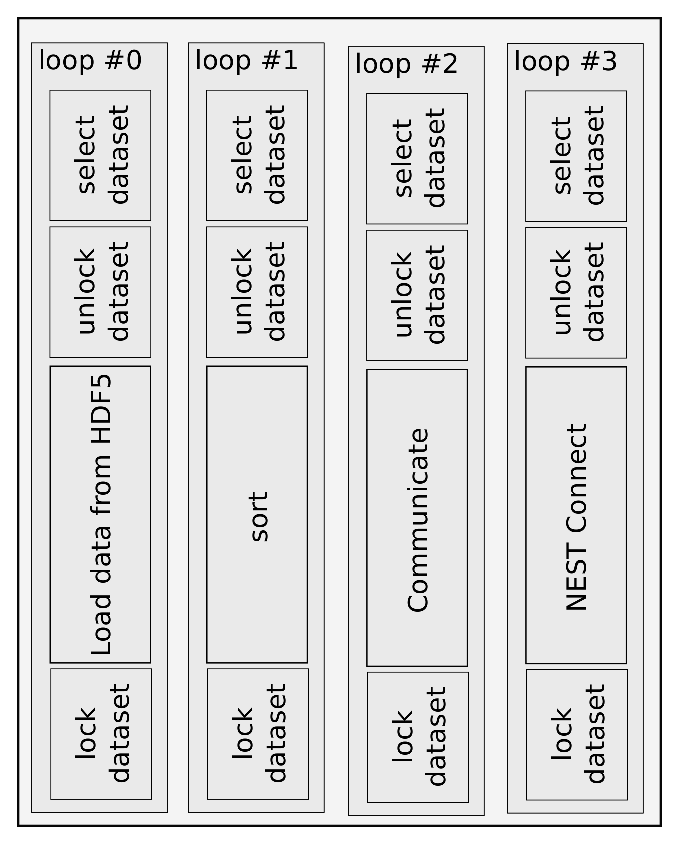
\includegraphics[scale=0.5]{alg_hybrid.eps}
	\caption{Hybrid implementation of algorithm. Each column is executed on another thread. 
	The selection of the datasets works in a round robin fashion.
	Thus the order of applied tasks on each dataset is equal to the sequential algorithm.
	The unblock call can block a thread, if the selected dataset is still in use by the previous thread.}
	\label{Mikesformatcon}
\end{figure}


\subsubsection{memory consumption}
\begin{figure}[h]
\begin{tabular}{| l | l | l | l |}
    \hline
    (id) & data structures & memory consumption \\ \hline
    (0) & neuron flags & $ non * BYTE $ \\ \hline
    (1) & chunk in memory & $ny (nx+1) * INT$ \\ \hline
    (2) & synapse table & $ c * 3INT $ \\ \hline
    (4) & MPI send vectors & $ c * 3INT $ \\ \hline
    (5) & MPI recv vectors & $ \frac{c}{\nu} * 3INT $ \\ \hline
    \end{tabular}
\caption{$non$: number of neurons; $ny$: number of columns of HDF5 datasets; $nx$: number of rows of HDF5 datasets $c$: parameter for size of table; $\nu$: distribution coefficient of data}
\end{figure}

\begin{equation}
  M = non * BYTE + 4*(c * 3INT) + c * 3INT + \frac{c}{\nu} * 3INT + ny (nx+1) * INT
  \label{eq:c++maxmemoryconsumption}
\end{equation}
The parameter $c$ allows a variation of memory consumption of the algorithm.
Besides the algorithm the memory consumption of NEST increases with the amount of created synapses.
The impact of $c$ to the runtime has to investigated to come up with reasonable variations of $c$.

\newpage
\section{Transpose data before send}
The algorithm needs a list of HDF5 files and the chunk size.
\begin{algorithm}
	\KwData{List of HDF5 files for each node, chunk size}
	\KwResult{Connected NEST network}
	\While{Chunk to read in HDF5 files}{
		Read chunk and store in memory\;
		Transpose data\;
		Map target neurons to nodes\;		
		MPI\_Alltoall transposed data\;
		%\For{Nodes}{
		%	Gather connections to node depending on target map
		%}
		Connect own connections in NEST\;
	}
\label{alg}
\caption{Distribute connection information}
\end{algorithm}


\begin{algorithm}/
	\KwData{Connection map [$S_1$ - [$T_1$,$T_2$,..], $S_2$ - ..]}
	\KwResult{Transposed connection map}
	Extract map to table [[$S_1$, $T_1$],[$S_2$, $T_2$],..]\;
	Sort table by target neurons\;
	Shrink table to map [$T_1$ - [$S_1$,$S_2$,..], $T_2$ - ..]\;		
\label{transdata}
\caption{Transpose data, $S_i$ source neuron $i$, $T_i$ target neuron $i$}
\end{algorithm}

\subsection{Memory consumption}
\begin{figure}[h]
\begin{tabular}{| l | l | l | l |}
    \hline
    data structures & memory consumption \\ \hline
    chunk in memory & $L_0 + h*(L_0 + L_S*w)$ \\ \hline
    connection map & $2*L_0+L_0*h+L_S*w*h$ \\ \hline
    tmp map for transposing & $2*L_0+2*L_S*w*h$ \\ \hline
    transposed con map & $2*L_0+L_0*(w*h-DNC)+L_S*w*h$ \\ \hline
    target node map & $L_0 + L_S*(w*h-DNC)$ \\ \hline
    own con map & $(2*L_0+L_0*(w*h-DNC)+L_S*w*h)/\nu$ \\ \hline
    \end{tabular}
\caption{$L_0$: constant memory overhead of list; $L_S$: memory consumption of entry type; $w$: 1 dim of chunk; $h$: 2 dim of chunk; $DNC(w)$: replication of target neurons in chunk; $\nu$: distribution coefficient of data}
\end{figure}	

\section{Memory consumption of NEST}
The memory usage of the newest NEST release 2.6.0 can be calculated with following equation. \cite{kunkel2014spiking}
\begin{equation}
  \Pi(M,T,N,K) =  \Pi_0 + \Pi_n(M,N)  + \Pi_c(M,T,N,K)
  \label{eq:NESTmemconsumption}
\end{equation} 
\begin{equation}
  \Pi_n(M,N) = N_M*1124
\end{equation}
\begin{equation}
  \Pi_c(M,T,N,K) = 0.33 * T * N + T * N^1_c * 24 + T*(N-N^1_c)*128 + N_M*K*16
\end{equation}
$\Pi$ is the memory consumption. $\Pi_0$ is the initial memory consumption of NEST.
For the \emph{JUQUEEN} its around 26 MB and for \emph{K} around 260 MB.
$M$,$T$, $N$, $K$ correspond to number of MPI Nodes, number of threads per node, number of neurons and number of outgoing connection per neuron.
For the calculation there are some simplifications done.
The model uses the \emph{iaf\_psc\_alpha} neuron model for all neurons. There are only static synapses.
The number of incoming connection per neuron $K$ is not known. Only the number of outgoing connections is known.
To get some results anyway, it is expected that they are similar. At this point a worse case analysis should be done!!
Furthermore the term of expected number of neurons without any VP-local target is set to zero, which is the worst case for the consumption of memory.
\begin{figure}[h]
\centering
\includegraphics[scale=0.5]{predicted_mem_NEST.eps}
	\caption{$T=8$, $K=2500$, $N=80,000,000$}
	\label{Mikesformatcon}
\end{figure}

\begin{figure}[h]
\centering
\includegraphics[scale=0.5]{Mikes_con_format.eps}
	\caption{Connection information for a neuronal network are given in HDF5 files.
The HDF5 files contain datasets which stores connection information grouped by the location of the source (pre-synaptic) neuron.
Each dataset contains a table:
Each column contains the connection information for the source (pre-synaptic) neuron.
Each first cell in the column contains the source neuron id.
The following cells contain the target (post-synaptic) neuron ids.}
	\label{Mikesformatcon}
\end{figure}

\section{Optimized data format for NEST}
The data format descripted in \ref{Mikesformatcon} contains connection information based on source and target ids.
There are no more synapsis information as synaptic type and biochemical constants available.
Synaptic types which depends on the source neuron type can be generated by a random distribution on the fly.
But the synaptic delay depends on the distance of the source and target neuron, which are stored in a seperate hdf5 file.
Therefore look up is nessecary which can be done in memory or disk.
First one is expensive in regards to time and the second one is expensive in regards to memory consumption.

\newpage
\section{Optimization strategies of current implementation}
The current implementation V03 allows to load all given data in parallel on 1K nodes.
To get a meaningful neuronal network the given data has to be extended by the proportion of excitatory and inhibitory neurons.
The given dataset does not distinguish between both types.
Therefore all neurons are spitted up using a random function.
Further the synaptic delays of the connections has to be calculated.
They depend on the length of the connection.
Therefore the coordinates of the neurons are used to calculate each distance.
These distances are multiplied by an factor to get the synaptic delays.

A load-balancing strategy is implemented, which sorts all hdf5 files by size before they are distributed to the nodes.

Using the implementation inside NEST, it takes around 1 hour to build up the network. Simulating the whole network takes around 1,5 h per 1 second of real time.


\begin{figure}[ht!]
     \begin{center}
        \subfigure[Load hdf5 files]{%
            \label{fig:first}
            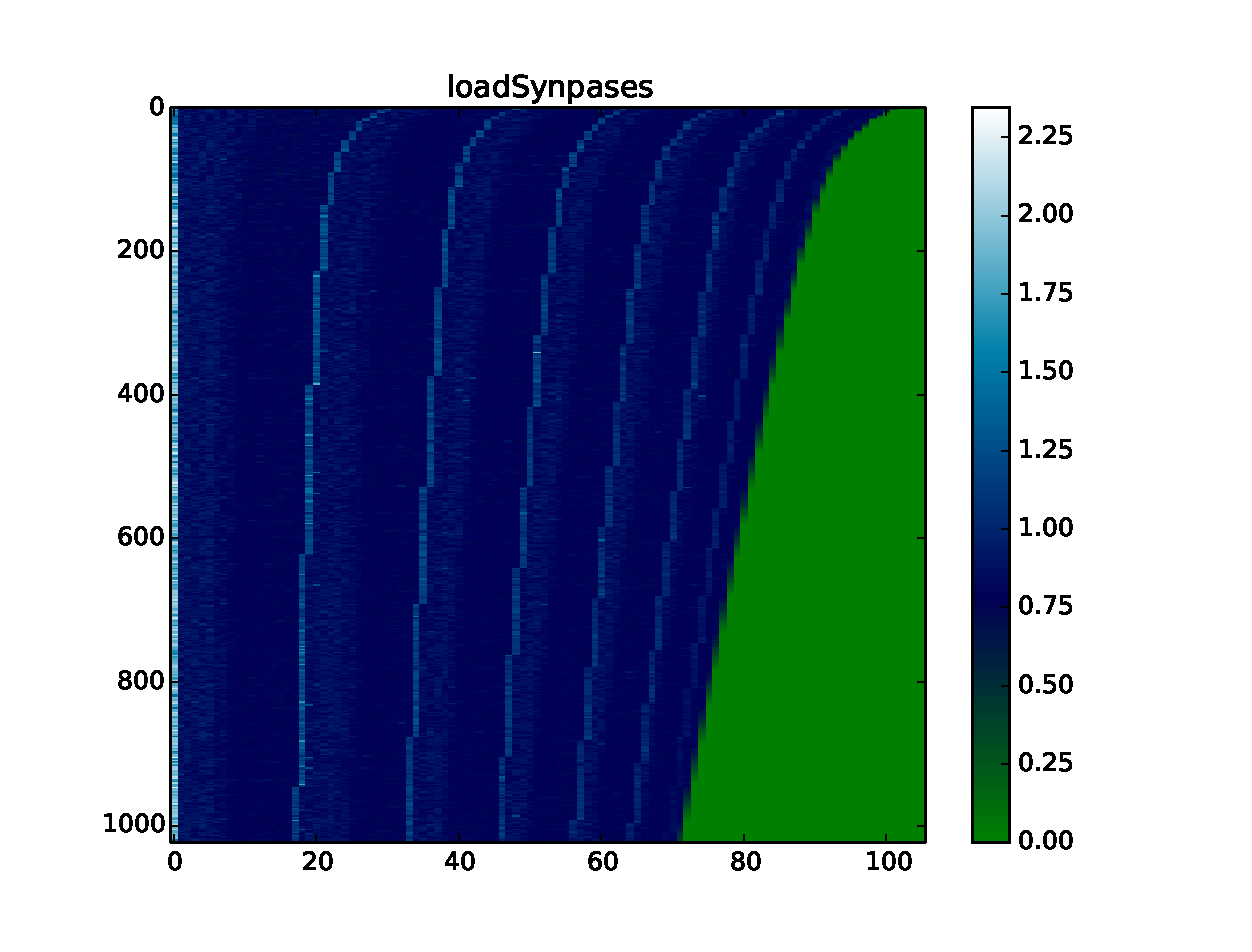
\includegraphics[width=0.4\textwidth]{V03_loadSynapses.eps}
        }
        \subfigure[Sort connection information data by target node]{%
           \label{fig:second}
           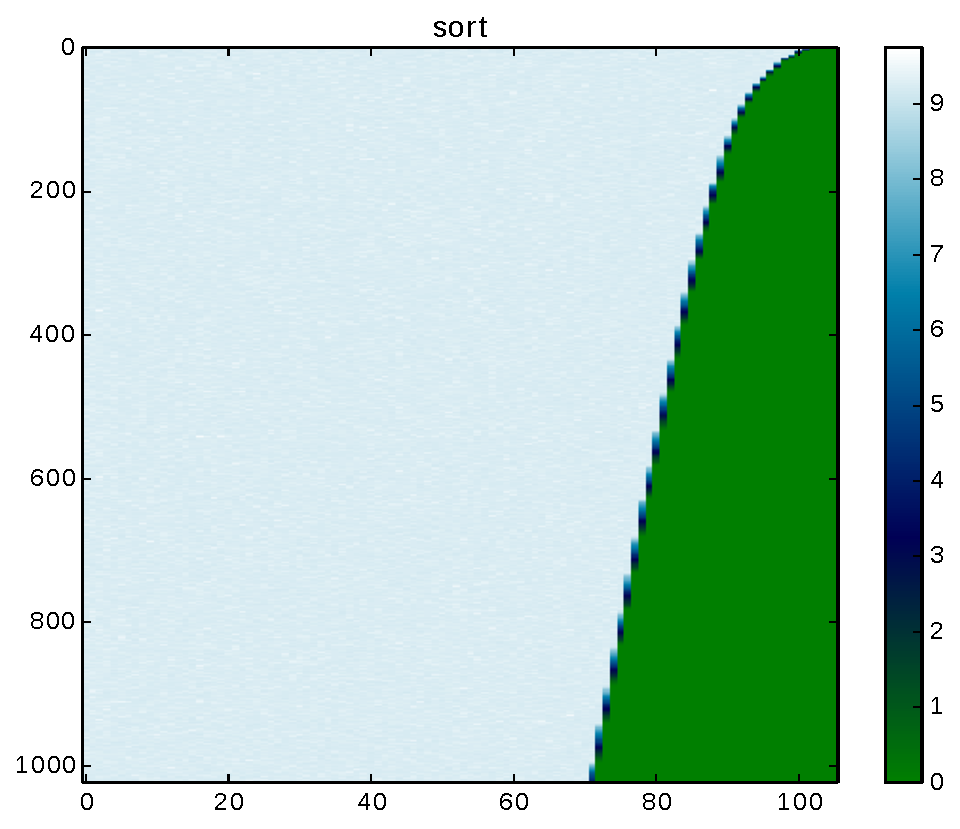
\includegraphics[width=0.4\textwidth]{V03_sort.eps}
        }\\ %  ------- End of the first row ----------------------%
        \subfigure[Send data to all target nodes using AlltoAllv]{%
            \label{fig:third}
            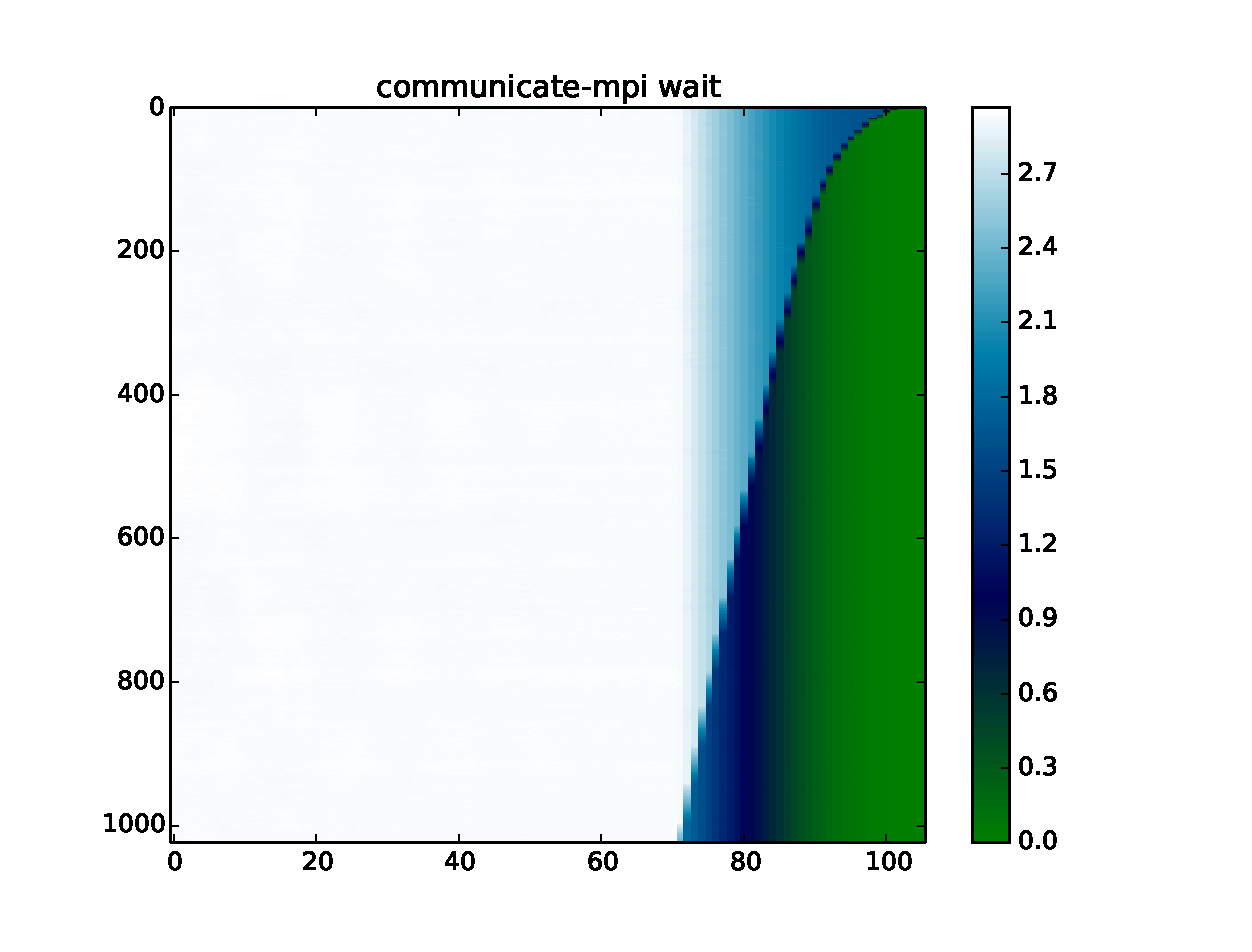
\includegraphics[width=0.4\textwidth]{V03_communicate.eps}
        }
        \subfigure[Connect function which calculated delay and calls NEST connect]{%
            \label{fig:fourth}
            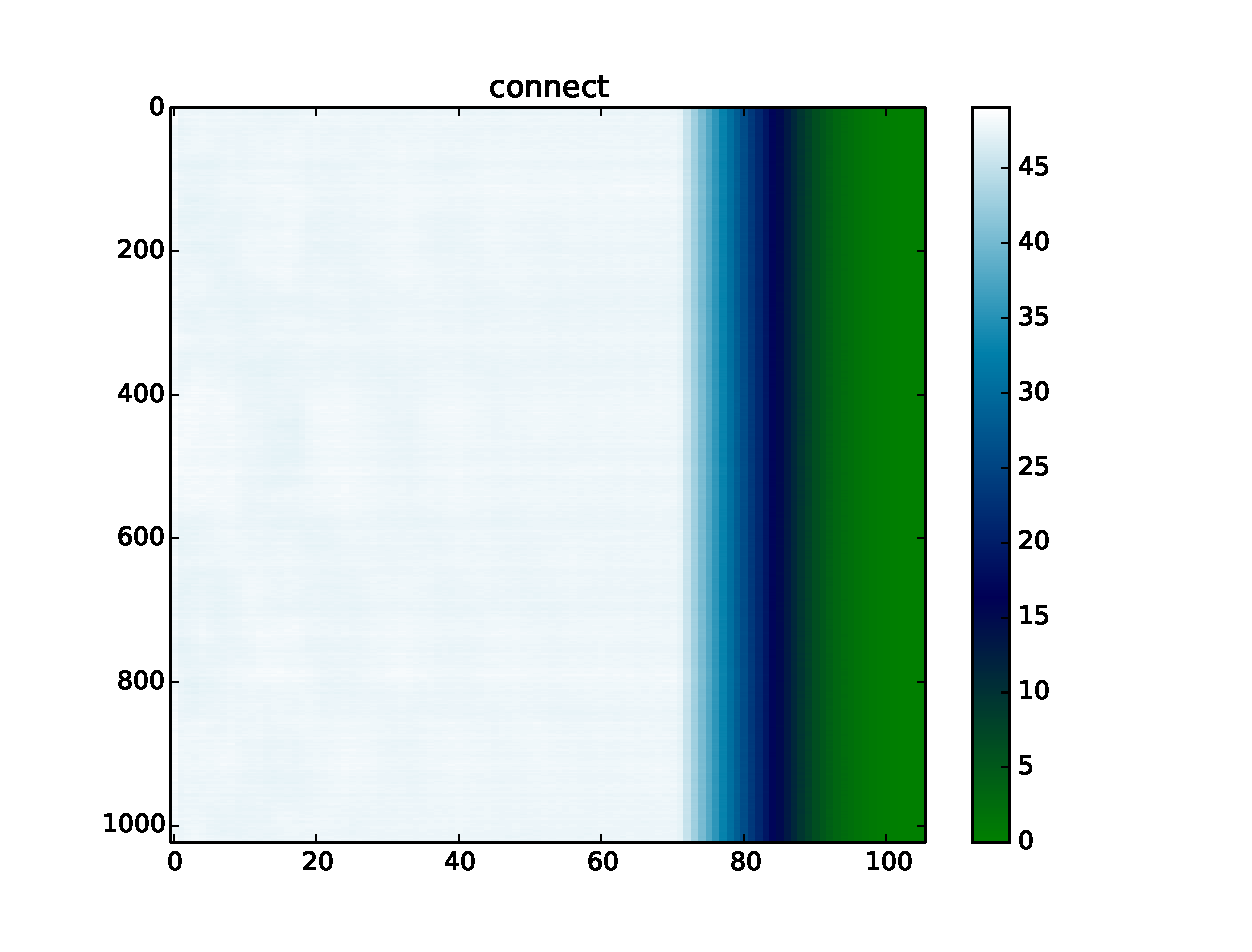
\includegraphics[width=0.4\textwidth]{V03_connect.eps}
        }
    \end{center}
    \caption{%
        The the plots show the the execution time for node per iteration.
        The y-axes corresponds to the node id and the x-axes corresponds to the iteration number.
        The color scale is in seconds.
        In each iteration loadSynapses loads max $1e6$ synapses from hdf5 file.
     }%
   \label{fig:implV03}
\end{figure}

\begin{figure}[ht!]
	\begin{center}
      	\label{fig:fourth}
    		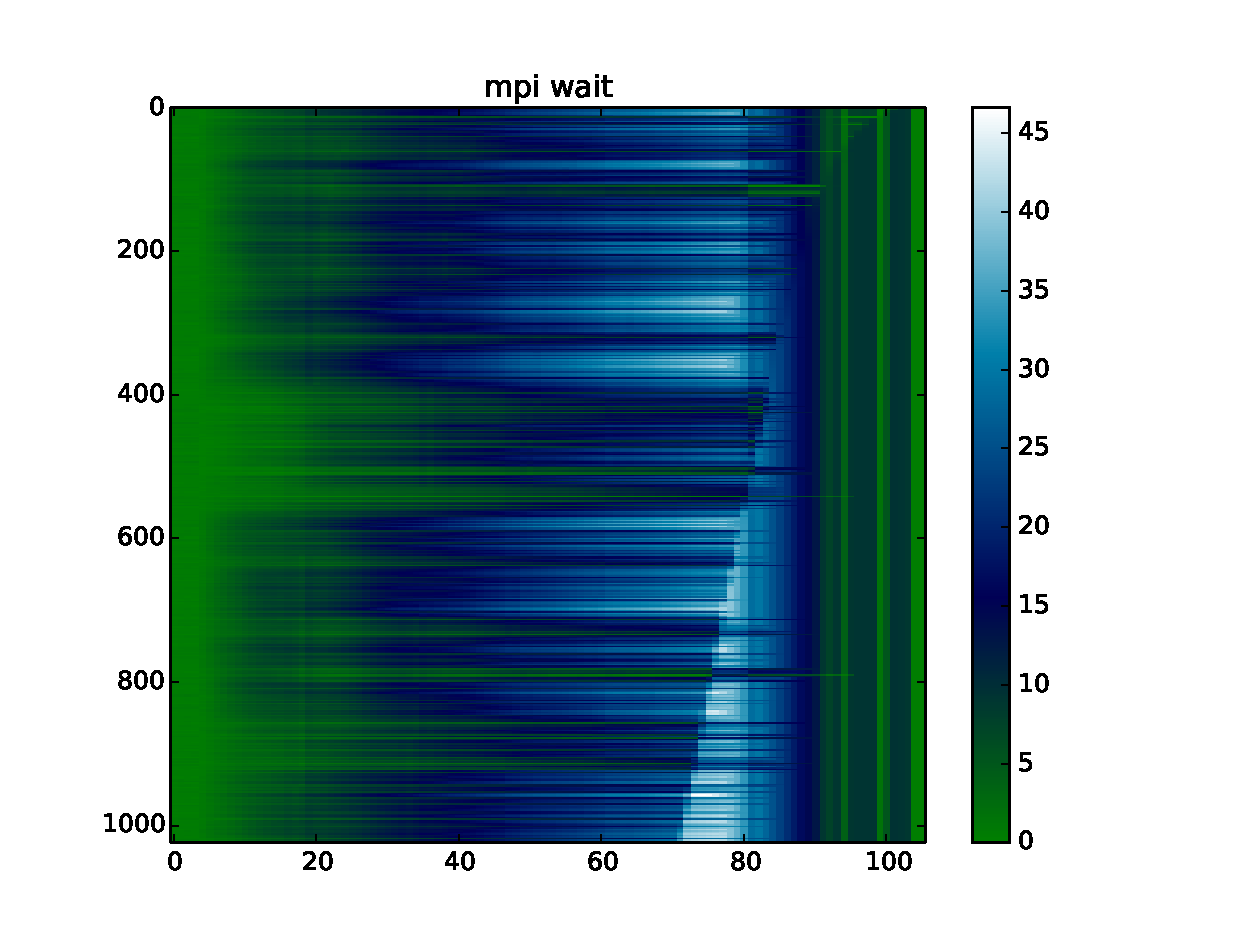
\includegraphics[width=0.6\textwidth]{V03_mpiwait.eps}
    		\caption{mpi wait}
    \end{center}
\end{figure}     


\subsection{Thread scheduling}
The current implementation uses mutexes to realize a task queue which runs in parallel on four different threads using four different datasets. So each thread handles one dataset. After a task is done on a thread the dataset is send in a round robin fashion to the next thread in the queue. The chosen strategy works fine on the BGQ, but violates the OpenMP standard.
Therefore a different queuing strategy should be implemented. An alternative approach is tested in an example program,
but not tested yet with the NEST implementation.

\subsection{Multi threaded call of NEST connect function}
In the current implementation the NEST connection function call takes most of the time.
It could be optimized calling it in parallel. Therefore another sorting operation has to be implemented.
The usage of parallel connect is critical and has to be tested carefully.
From a first look inside the code, it should be doable.
In the current implementation the NEST connect call takes around $25 \mu s$ per connection. 
 


\newpage
\bibliographystyle{plain}

\bibliography{./transpose_via_mpi}

\end{document}
